% !TEX encoding = UTF-8 Unicode
\documentclass{article}

\usepackage{polski}
\usepackage[utf8]{inputenc}
\usepackage{subfig}
\usepackage{graphicx}

\usepackage[a4paper, left=2.5cm, right=2.5cm, top=3.5cm, bottom=3.5cm, headsep=1.2cm]{geometry}

\linespread{1.3}

\begin{document}
	
	\begin{titlepage}
		\centering
		{\scshape\LARGE Politechnika Wrocławska \par}
		{\scshape\Large Katedra Informatyki Technicznej\par}
		
		\vspace{1.5cm}
		{\scshape\Huge Bazy Danych \par}
		\vspace{1.5cm}
		
		\vspace{2cm}
		{\Large\itshape Magdalena Biernat\par}
		{\Large\itshape Mateusz Bortkiewicz\par}
		\vfill\flushleft\large
		
		\normalsize	\centering	\vspace{3cm}
		Prowadzący\par
		dr inż. Tomasz Janiczek 
		
		\vfill
		{\large \today\par}
	\end{titlepage}
	\newpage
	\section{Model konceptualny bazy danych}
	\begin{figure}[!ht]	
		\centering
		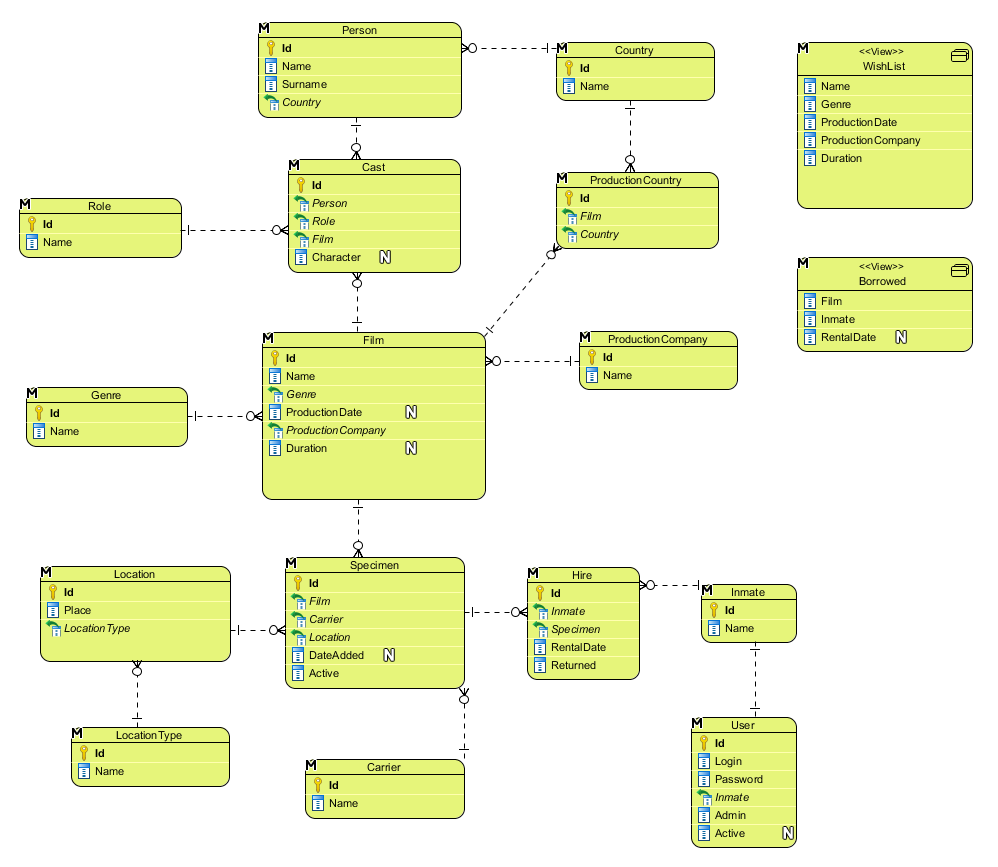
\includegraphics[height=13cm]{model_konceptualny.png}
		\caption{Model konceptualny}
		\label{fig:obrazek 0}
	\end{figure}
	\newpage
	\section{Opis "świata rzeczywistego"}
	Opis "świata rzeczywistego" - aplikacja "Domowa wypożyczalnia wideo"
	\subsection{Opis zasobów ludzkich}
		- Głowa rodziny, tudzież osoba wyznaczona w domu administruje i zarządza aplikacją desktopową "Domowa wypożyczalnia wideo". Może ona usuwać i dodawać użytkowników, resetować hasła, zwracać/wypożyczać administracyjnie egzemplarze filmów, usuwać tytuły filmów, wycofywać z użycia egzemplarze filmów, a także wykonywać to co zwykły użytkownik
		- Użytkownik, mieszkaniec domostwa może dodać lub edytować tytuły filmów oraz egzemplarze do tytułów obecnych już filmów. Może wypożyczać dostępny egzemplarz filmu
		- Wypozyczenie posiada identyfikator domownika, identyfikator egzemplarza filmu a także datę wypożyczenia i informację czy film jest zwrócony.
		- Użytkownik może edytować swoje konto, tj. zmieniać hasło.
	\subsection{Przepisy}
		Liczba wypożyczonych jednocześnie egzemplarzy przez danego użytkownika nie może być większa niż trzy. Nie istnieje termin zwrotu - wypożyczenie jest bezterminowe. Nieaktywny użytkownik nie może się zalogować na konto i wypożyczyć/zwrócić filmu.
	\subsection{Dane techniczne}
	\label{dane_techniczne}
		 Obsługa konta, bazy wideo i wypożyczeń powinna być dostępna przez aplikację desktopową połączoną z bazą danych.
		Wypożyczający loguje się do konta za pomocą loginu i hasła. Hasło nie jest przechowywane w bazie danych (jest to jedynie zahaszowane hasło).
	\newpage
	\section{Wymagania funkcjonalne i niefunkcjonale}
	\subsection{Wymagania funkcjonalne}
	\begin{itemize}
	\item aplikacja ma mieć możliwość wyszukiwania\$dodawania\$edytowania\$usuwania filmów do bazy danych
	\begin{itemize}
		\item wyszukiwać i dodawać filmy może każdy użytkownik
		\item usuwać i edytować może tylko administrator systemu
	\end{itemize}
	\item aplikacja ma mieć możliwość edytowania danych użytkownika
	\item  dodawać nowego użytkownika może tylko administrator
	\item aplikacja ma mieć możliwość wyszukiwania\$dodawania\$edytowania\$usuwania tytułów filmów do bazy danych 
	\begin{itemize}
		\item wyszukiwać i dodawać tytuły może każdy użytkownik
		\item usuwać i edytować może tylko administrator systemu
	\end{itemize}
	\item obsadę może dodawać każdy użytkownik
	\item aplikacja pokazuje wypożyczone pozycje i listę życzeń (filmy, których egzemplarze nie są umieszczone w bazie danych)
	\end{itemize}
	\subsection{Wymagania niefunkcjonalne}	
	\begin{itemize}
		\item ilość domowników nie wpływa na szybkość działania systemu
		\item ilość filmów/tytułów/użytkowników etc. Jest ograniczona tylko pojemnością dysku na którym stoi baza danych
		\item przyjazny interfejs użytkownika
		\item liczba błędów w aplikacji przez pierwszy miesiąc od wydania aplikacji nie może przekroczyć 5		
	\end{itemize}
\newpage
	\section{Diagram przypadków użycia}
	\begin{figure}[!ht]	
		\centering
		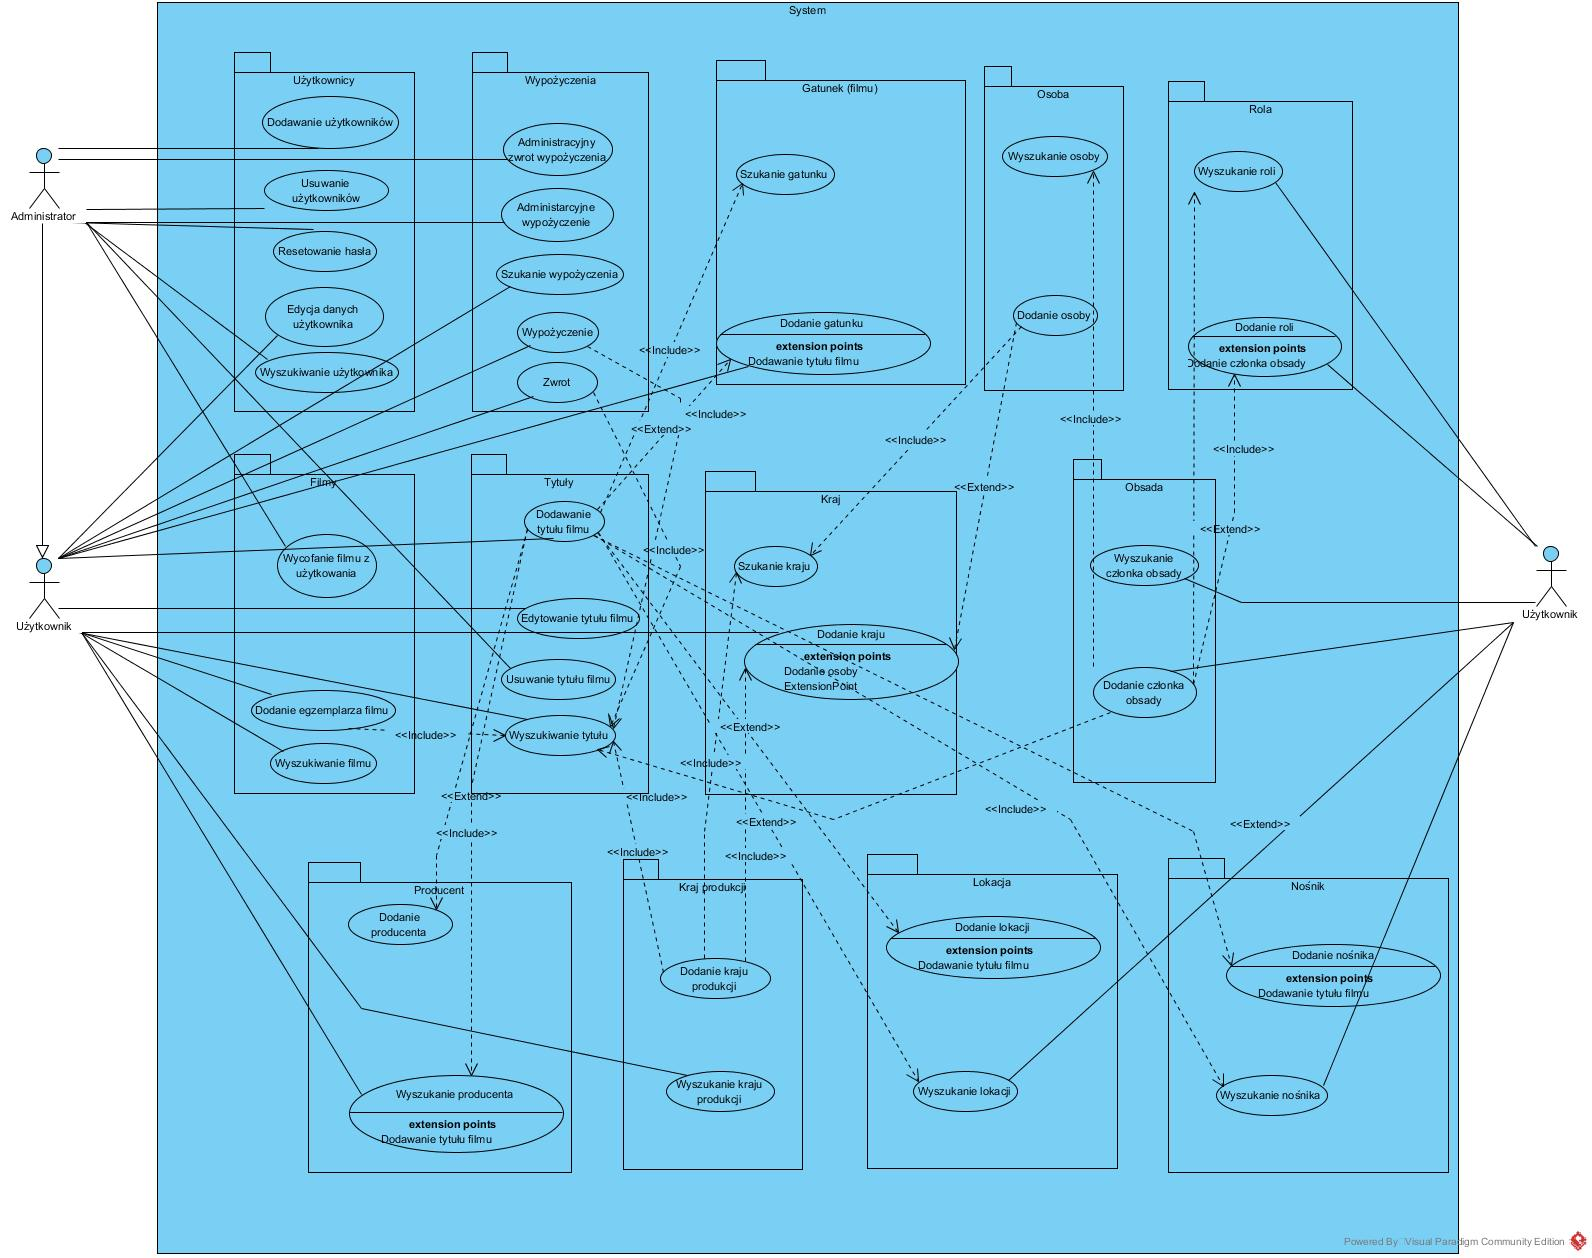
\includegraphics[height=13cm]{PU.jpg}
		\caption{Diagram PU}
		\label{fig:obrazek 1}
	\end{figure}
\newpage
	\section{Diagram związków encji}
		\begin{figure}[!ht]	
		\centering
		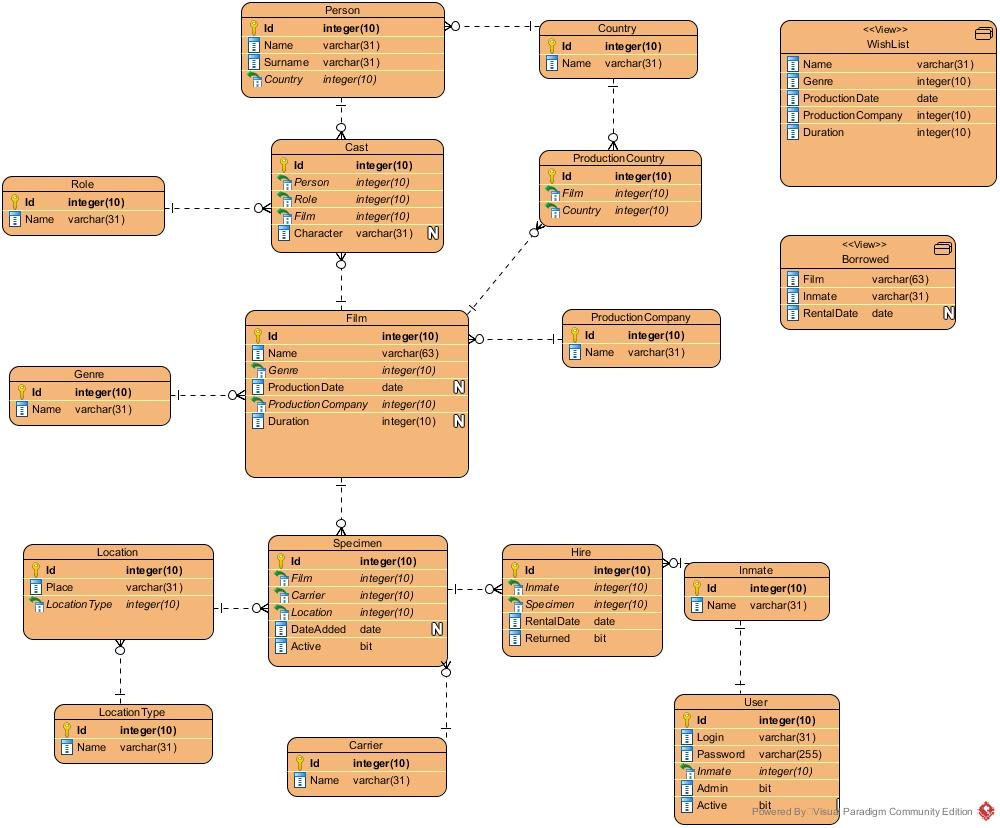
\includegraphics[height=14cm]{diagram_zwiazkow_encji.jpg}
		\caption{Diagram związków encji}
		\label{fig:obrazek 2}
	\end{figure}
\newpage
\section{Analiza ilości encji}
\subsection{Analiza liczby instancji dla każdej encji}
\begin{itemize}
\item Film – ok. 50 rekordów (przykładowo)
\item Specimen – ok. 50 rekordów (podobnie jak Film)
\item Carrier (nośnik) – 5-10 rekordów ( Nie więcej jak Specimen)
\item LocationType (typ lokacji) – 5-10 rekordów (nie więcej jak Location)
\item Location (lokacja) – ok. 50 rekordów (nie więcej jak Specimen)
\item Hire (wypożyczenie) – 10 na sam początek , nie więcej jak 3 * liczba użytkowników
\item Inmate (domownik) – ok. 10 rekordów
\item User (użytkownik) – ok.10 rekordów (tak samo jak Inmate)
\item ProductionCompany (Wytwórnia filmów) – ok. 10-15 rekordów
\item Person (osoba)– minimalnie ilość rekordów 1 per Film (przykładowo)
\item Cast (obsada) – maksymalnie Person * Role * Film
\item Role (rola w filmie) – ok. 10 rekordów (przykładowo)
\item Contry (kraj) – maksymalnie ok. 240, minimalnie 1
\item ProductionCountry (Kraj produkcji) – maksymalnie Contry * Film
\item Genre (gatunek) – ok. 15 rekordów (przykładowo)
\end{itemize}

\subsection{Analiza użycia dla każdej encji}
\begin{itemize}
\item Film – wyszukiwanie najczęściej, potem dodawanie i edycja, prawie wcale usuwanie
\item Specimen - wyszukiwanie najczęściej, potem dodawanie i edycja, prawie wcale usuwanie
\item Carrier – wyszukiwanie najczęściej, rzadziej dodawanie (najwięcej rekordów na początku istnienia bazy), prawie wcale edycja, brak usuwania
\item LocationType – wyszukiwanie najczęściej, potem dodawanie, brak usuwania i edycji
\item Location – wyszukiwanie najczęściej, podobnie dodawanie, najmniej edycja, brak usuwania
\item Hire – wyszukiwanie i dodawanie najczęściej, podobnie usuwanie, brak edycji
\item Inmate – wyszukiwanie najczęściej, rzadziej dodawanie, brak edycji i usuwania
\item User – wyszukiwanie najczęściej, rzadziej dodawanie i edycja, brak usuwania
\item ProductionCompany – wyszukiwanie najczęściej, potem dodawanie, brak edycji i usuwania
\item Person – wyszukiwanie najczęściej, potem dodawanie, brak edycji i usuwania
\item Cast – najczęściej wyszukiwanie, potem dodawanie, brak edycji, rzadko usuwanie
\item Role – najczęściej wyszukiwanie, rzadko dodawanie (najwięcej rekordów na początku istnienia bazy), brak edycji i usuwania
\item Country – najczęściej wyszukiwanie, rzadko dodawanie, (najwięcej rekordów na początku istnienia bazy) brak edycji i usuwania
\item ProductionCountry  - najczęściej wyszukiwanie, potem dodawanie, rzadko edycja, brak usuwania
\item Genre – najczęściej wyszukiwanie, rzadko dodawanie (najwięcej rekordów na początku istnienia bazy), brak usuwania i edycji

\end{itemize}
\section{Implementacja bazy danych}
\subsection{Serwer bazodanowy}
W związku z chęcią realizacji aplikacji na platformie .NET, zdecydowaliśmy się na wybór instancji bazodanowej dostarczonej przez firmę Microsoft, a mianowicie MS SQL Server w wersji 2014. Do jej zarządzania będziemy używać dostarczonego w pakiecie narzędzia - Management Studio, bądź też przeglądarki wbudowanej w środowisko programistyczne - Visual Studio 2015.
\subsection{Tworzenie tabel i insertowanie danych}
Tabele stworzono wg diagramów związków encji. Zawierają one przykładowe dane, niekoniecznie zgodne z rzeczywistością. Dla ułatwienia, tabeli zawierającej wypożyczenia, a także pola HashedPassword w tabeli Users nie wypełniono - będą one użyte, jak również wypełnione, podczas testów aplikacji w etapie III. Skrypt tabeli zamieszczony jest w załączniku.
\section{Polityka bezpieczeństwa}
\subsection{Zabezpieczenie serwera}
W celu zwiększenia bezpieczeństwa, dostęp do instancji bazodanowej będzie chroniony, tzn. aby się z nią połączyć potrzebne będzie hasło. Na potrzebny budowania aplikacji i testów, instancja bazodanowa nie będzie posiadać hasła. 
\subsection{Dostęp do kont użytkowników}
Jak to zostało wspomniane w danych technicznych w punkcie \ref{dane_techniczne}, hasła użytkowników planujemy szyfrować. Myślimy o wykorzystaniu szyfrowania symetrycznego. Jako iż będziemy korzystać z platformy .NET, do naszych celów wykorzystamy gotową klasę CryptoStream biblioteki System.Security.Cryptography, która pozwoli nam przekształcać hasło, na niezrozumiały ciąg znaków. Wykorzystuje ona szyfrowanie \textit{AES} (ang. Advanced Encryption Standard). 
\end{document}